\documentclass[12pt]{article}
\usepackage[utf8]{inputenc}

\usepackage{amsmath}
\usepackage{bookmark}
\usepackage[a4paper, margin=3.5cm]{geometry}
\usepackage{graphicx} % For inserting images
\usepackage{hyperref} % For hyperlinks
\usepackage{indentfirst}
\usepackage{minted} % For code-highlighting
\usepackage{parskip}

\graphicspath{ {./images/} }
\setlength{\parindent}{15pt} % Set paragraph indentation
\setlength{\parskip}{1em} % Set paragraph space (one line)
\setminted{frame=single, breaklines} % Set codeblock style

\title{Programming Practicum Report:\\Meeting \#6}
\author{\href{https://github.com/avaxar}{R. Ethan Halim}}
\date{October 14th, 2024}

\begin{document}

\maketitle

\section{Averaging Student Scores}
The entire source file is hosted on a GitHub repository \href{https://github.com/avaxar/uni-practica-1/tree/main/week_6/01_student_scores}{\textbf{here}}.

\subsection{Explanation}

The sole requirement of this assignment is the usage of a C++ struct in order to store each student's record. Below are the definition and the fields of the struct involved in the purpose thereof. Since the student ID might or might not contain non-numeral characters, I chose to use \texttt{std::string} as its data type to accommodate both.

\begin{minted}{cpp}
struct Student {
    std::string id;
    double midterm;
    double final;
    double average;
};
\end{minted}

Initially, the program requests the number of students to be inputted into the program. This will be used for the for-loop later on to receive the midterm and the final scores of the \texttt{n} students. Additionally, the program automatically exits and returns an error code if the number of students is zero.

\begin{minted}{cpp}
int program(std::istream& cin, std::ostream& cout) {
    size_t n_students;
    cout << "Enter the amount of students: ";
    cin >> n_students;

    // Exits early if the inputted number of students is zero.
    if (n_students == 0) {
        cout << "Provide at least one input!\n";
        return 1;
    }

    ...
}
\end{minted}

Using the received number of students, the for-loop below iterates for every student whose midterm and final score values are to be inputted into the vector of \texttt{Student} instances. On each iteration, the program provides the fields of each \texttt{Student} instance to be filled by the user: the student ID, the midterm exam score, and the final exam score.

\begin{minted}{cpp}
int program(std::istream& cin, std::ostream& cout) {
    ...

    std::vector<Student> students;
    cout << '\n';
    for (size_t i = 1; i <= n_students; i++) {
        Student student;
        cout << "[Data for Student #" << i << "]\n";

        // Gets the student ID (as a string)
        cout << "- ID: ";
        while (student.id.empty()) {
            std::getline(cin, student.id);
        }

        // Gets the midterm exam score
        while (true) {
            cout << "- Midterm exam score: ";
            cin >> student.midterm;

            // Loops again if the inputted score is invalid
            if (student.midterm > 100) {
                cout << "The score must not exceed 100!\n";
            }
            else {
                break;
            }
        }

        // Gets the final exam score
        while (true) {
            cout << "- Final exam score: ";
            cin >> student.final;

            // Loops again if the inputted score is invalid
            if (student.final > 100) {
                cout << "The score must not exceed 100!\n";
            }
            else {
                break;
            }
        }

        ...
    }

    ...
}
\end{minted}

Notice that there exist two of the template code below, whereby \texttt{[...]} refers to either the student's midterm score or final score. The code enclosed inside of the infinite while-loop ensures that the score inputted is within the range from 0 (by virtue of the underlying unsigned integer type used to store the score) to 100, as checked by the if-statement. If the user inputted a value outside of the said bounds, the program would ask them to reinput the value.

\begin{minted}{cpp}
while (true) {
    cout << "- [...] score: ";
    cin >> student.[...];

    // Loops again if the inputted score is invalid
    if (student.[...] > 100) {
        cout << "The score must not exceed 100!\n";
    }
    else {
        break;
    }
}
\end{minted}

\pagebreak
Finally, upon the conclusion of each iteration, the average score is computed from the given midterm and final scores, and stored in the field available in the \texttt{Student} struct. The structure instance is pushed into the vector.

\begin{minted}{cpp}
int program(std::istream& cin, std::ostream& cout) {
    ...

    for (size_t i = 1; i <= n_students; i++) {
        ...

        // Calculates the student average and pushes to the vector
        student.average = (student.midterm + student.final) / 2;
        students.push_back(student);
        cout << '\n';           }

    ...
}
\end{minted}

Once the data and the average score of each student have been gathered and calculated, they are all displayed at the end of the program. It iterates over the vector of \texttt{Student} instances, in order to announce their average scores sequentially. Additionally, the program calculates the overall average as well.

\begin{minted}{cpp}
int program(std::istream& cin, std::ostream& cout) {
    ...

    // Final output
    cout << "[Calculated Average(s) of All " << n_students << " Student(s)]\n";
    double sum;
    for (Student& student : students) {
        cout << "- Student ID #" << student.id << ": " << student.average << '\n';
        sum += student.average; // Sums each of the students' average score
    }
    cout << "The overall average is " << (sum / n_students) << ".\n";

    return 0;
}
\end{minted}

\pagebreak
\subsection{Manual Testing}
Below is the compilation and the testing of the source code.
\newline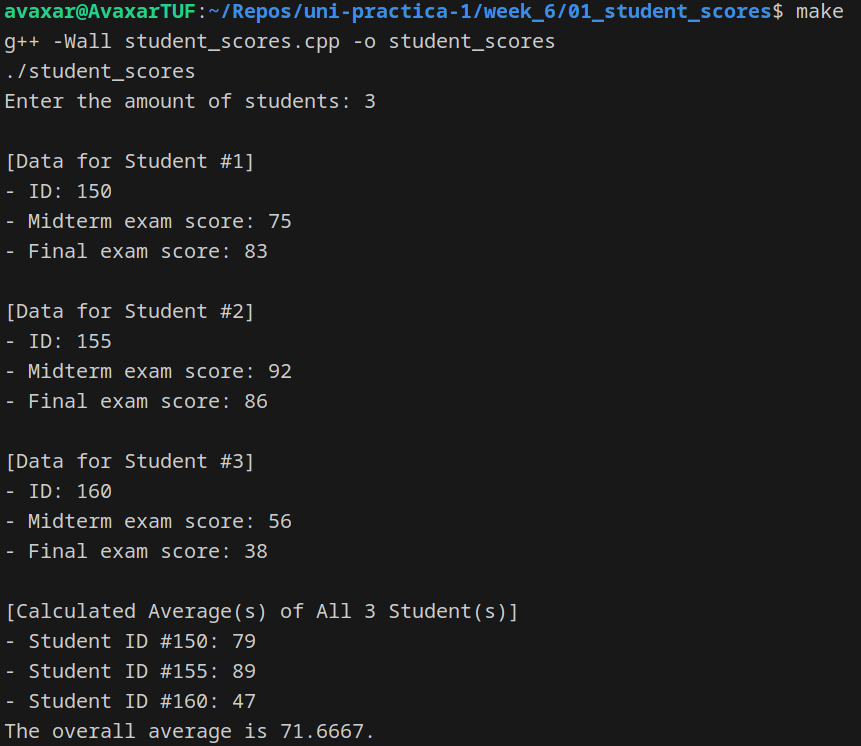
\includegraphics[width=\textwidth]{01_student_scores}

\pagebreak
\subsection{Test Cases}

\subsubsection{Tests}
Below is copied directly from the \texttt{tests.txt} file.
\inputminted{text}{01_student_scores/tests.txt}

\subsubsection{Execution}
Below are the results of the test cases. No test cases failed.
\newline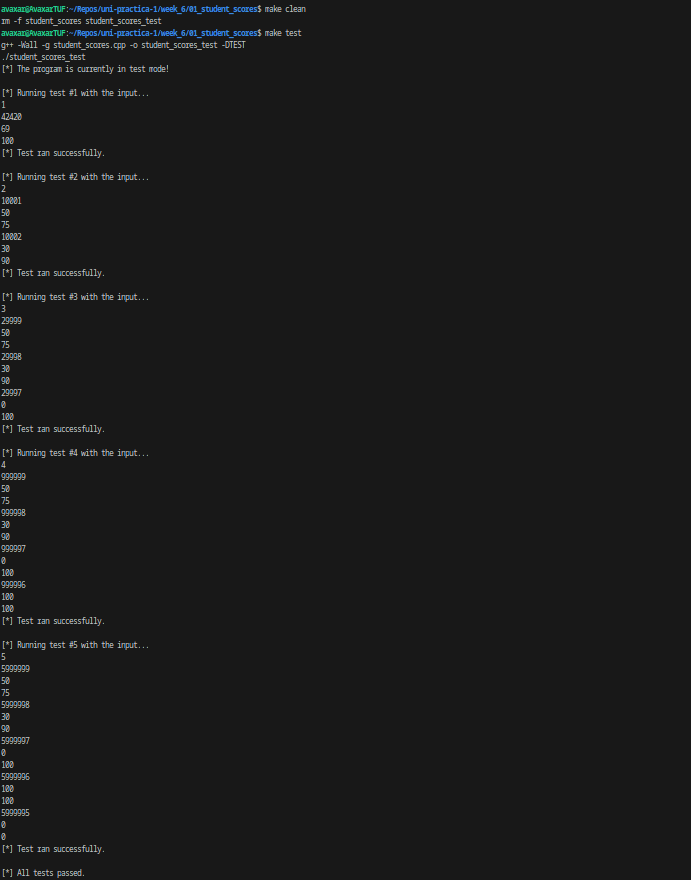
\includegraphics[width=\textwidth]{01_student_scores_test}

\end{document}
